\section*{k-Nearest Neighbors}

Remarks:

\begin{itemize}
  \item Different metrics can be employed
  \item High computational complexity for large $N$ (but efficient data structure may exist)
\end{itemize}

\subsection*{k-NN regression $(y \in \mathbb{R})$}
$
f_{S_{\text {train }}, k}(x)=\frac{1}{k} \sum_{n: x_{n} \in n b h_{S_{\text {train }, k}}(x)} y_{n}
$




\subsection*{k-NN classification $(y \in\{0,1\}$ )}
$
f_{S_{\text {train }, k}}(x)=\operatorname{majority}\left\{y_{n}: x_{n} \in \operatorname{nbh}_{S_{\text {train }, ~}}(x)\right\}
$


- Remarks:

\begin{itemize}
  \item Choose an odd value for $\mathrm{k}$ to prevent ties
  \item Generalization: smoothing kernels; weighted linear combination of elements
\end{itemize}

- Why does it make sense?
\begin{itemize}
  \item Relevant in the presence of spatial correlation

  \item Implicitly models intricate decision boundaries in low-dimensional spaces

\end{itemize}


\subsection*{Bias-variance tradeoff in k-NN}
For small k:

\begin{itemize}
  \item Low bias - complex decision boundary
  \item High variance - overfitting
\end{itemize}

For large k:

(When $k=N$, prediction is constant)

\begin{itemize}
  \item High bias
  \item Low variance
\end{itemize}


- 1-NN classification has max train acc


\subsection*{Summary: k-Nearest Neighbor}
Pros:
\begin{itemize}
  \item No optimization or training
  \item Easy to implement
  \item Works well in low dimensions, allowing for very complex decision boundaries
\end{itemize}

Cons:
\begin{itemize}
  \item Slow at query time
  \item Not suitable for high-dimensional data
  \item Choosing the right local distance is crucial
\end{itemize}


\subsection*{Curse of dimensionality}

\begin{wrapfigure}{r}{0.2\columnwidth} 
    \centering
    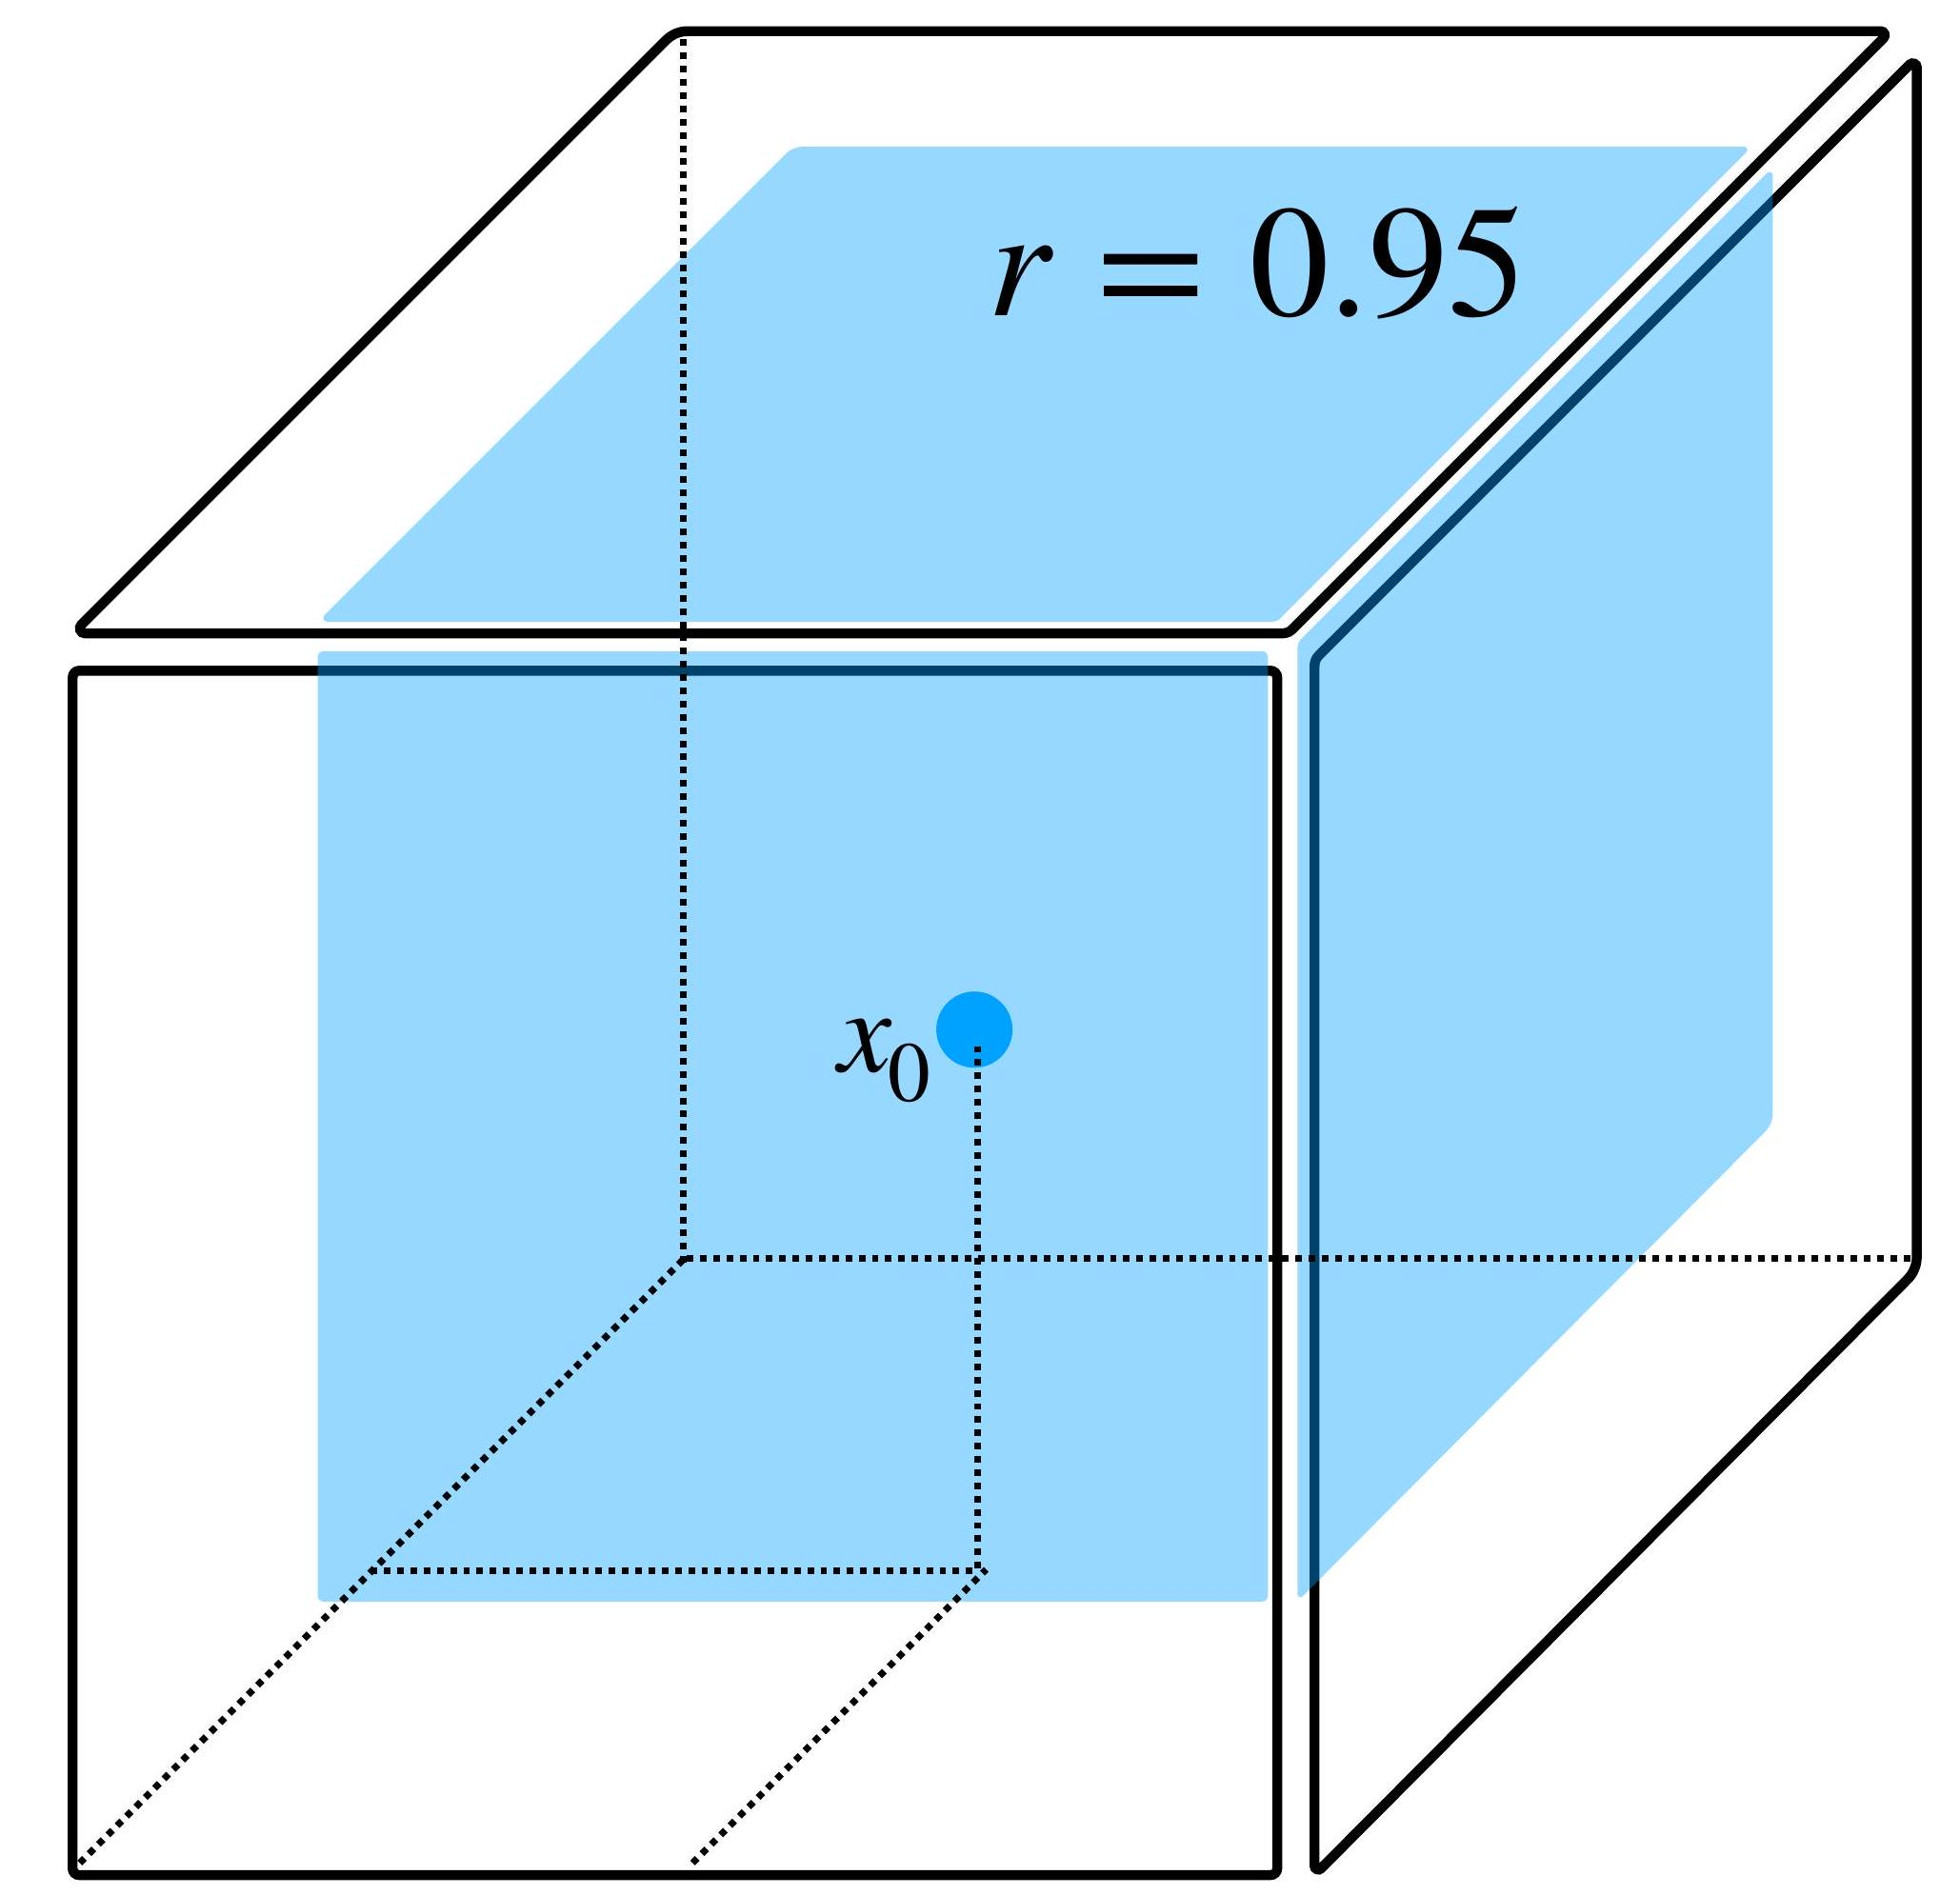
\includegraphics[width=0.2\columnwidth]{figures/dim_r=0_95.jpg}
    \text{\tiny{$\mathscr{X}=[0,1]^{d}$}}
\end{wrapfigure}

- \underline{Claim 1}: As the dimensionality grows, fixed-size training sets cover a diminishing fraction of the input space

- Assume the data $x \sim \mathcal{U}\left([0,1]^{d}\right)$

- Blue box around the center $x_{0}$ of size $r$

$
\mathbb{P}(x \in \mbox{\mancube})=r^{d}:=\alpha
$

- If $\alpha=0.01$, to have:
$
\begin{aligned}
& d=10, \text { we need } r=0.63 \\
& d=100, \text { we need } r=0.95
\end{aligned}
$

$d=100 \rightarrow$ need to explore almost the whole box


- \underline{Claim 2}: In high-dimension, data-points are far from each other.

- Consider $N$ i.i.d. points uniform in the $[0,1]^{d}$

$
\mathbb{P}\left(\exists x_{i} \in \mbox{\mancube}\right) \geq 1 / 2 \Longrightarrow r \geq\left(1-\frac{1}{2^{1 / N}}\right)^{1 / d}
$

\begin{wrapfigure}{r}{0.2\columnwidth} 
    \centering
    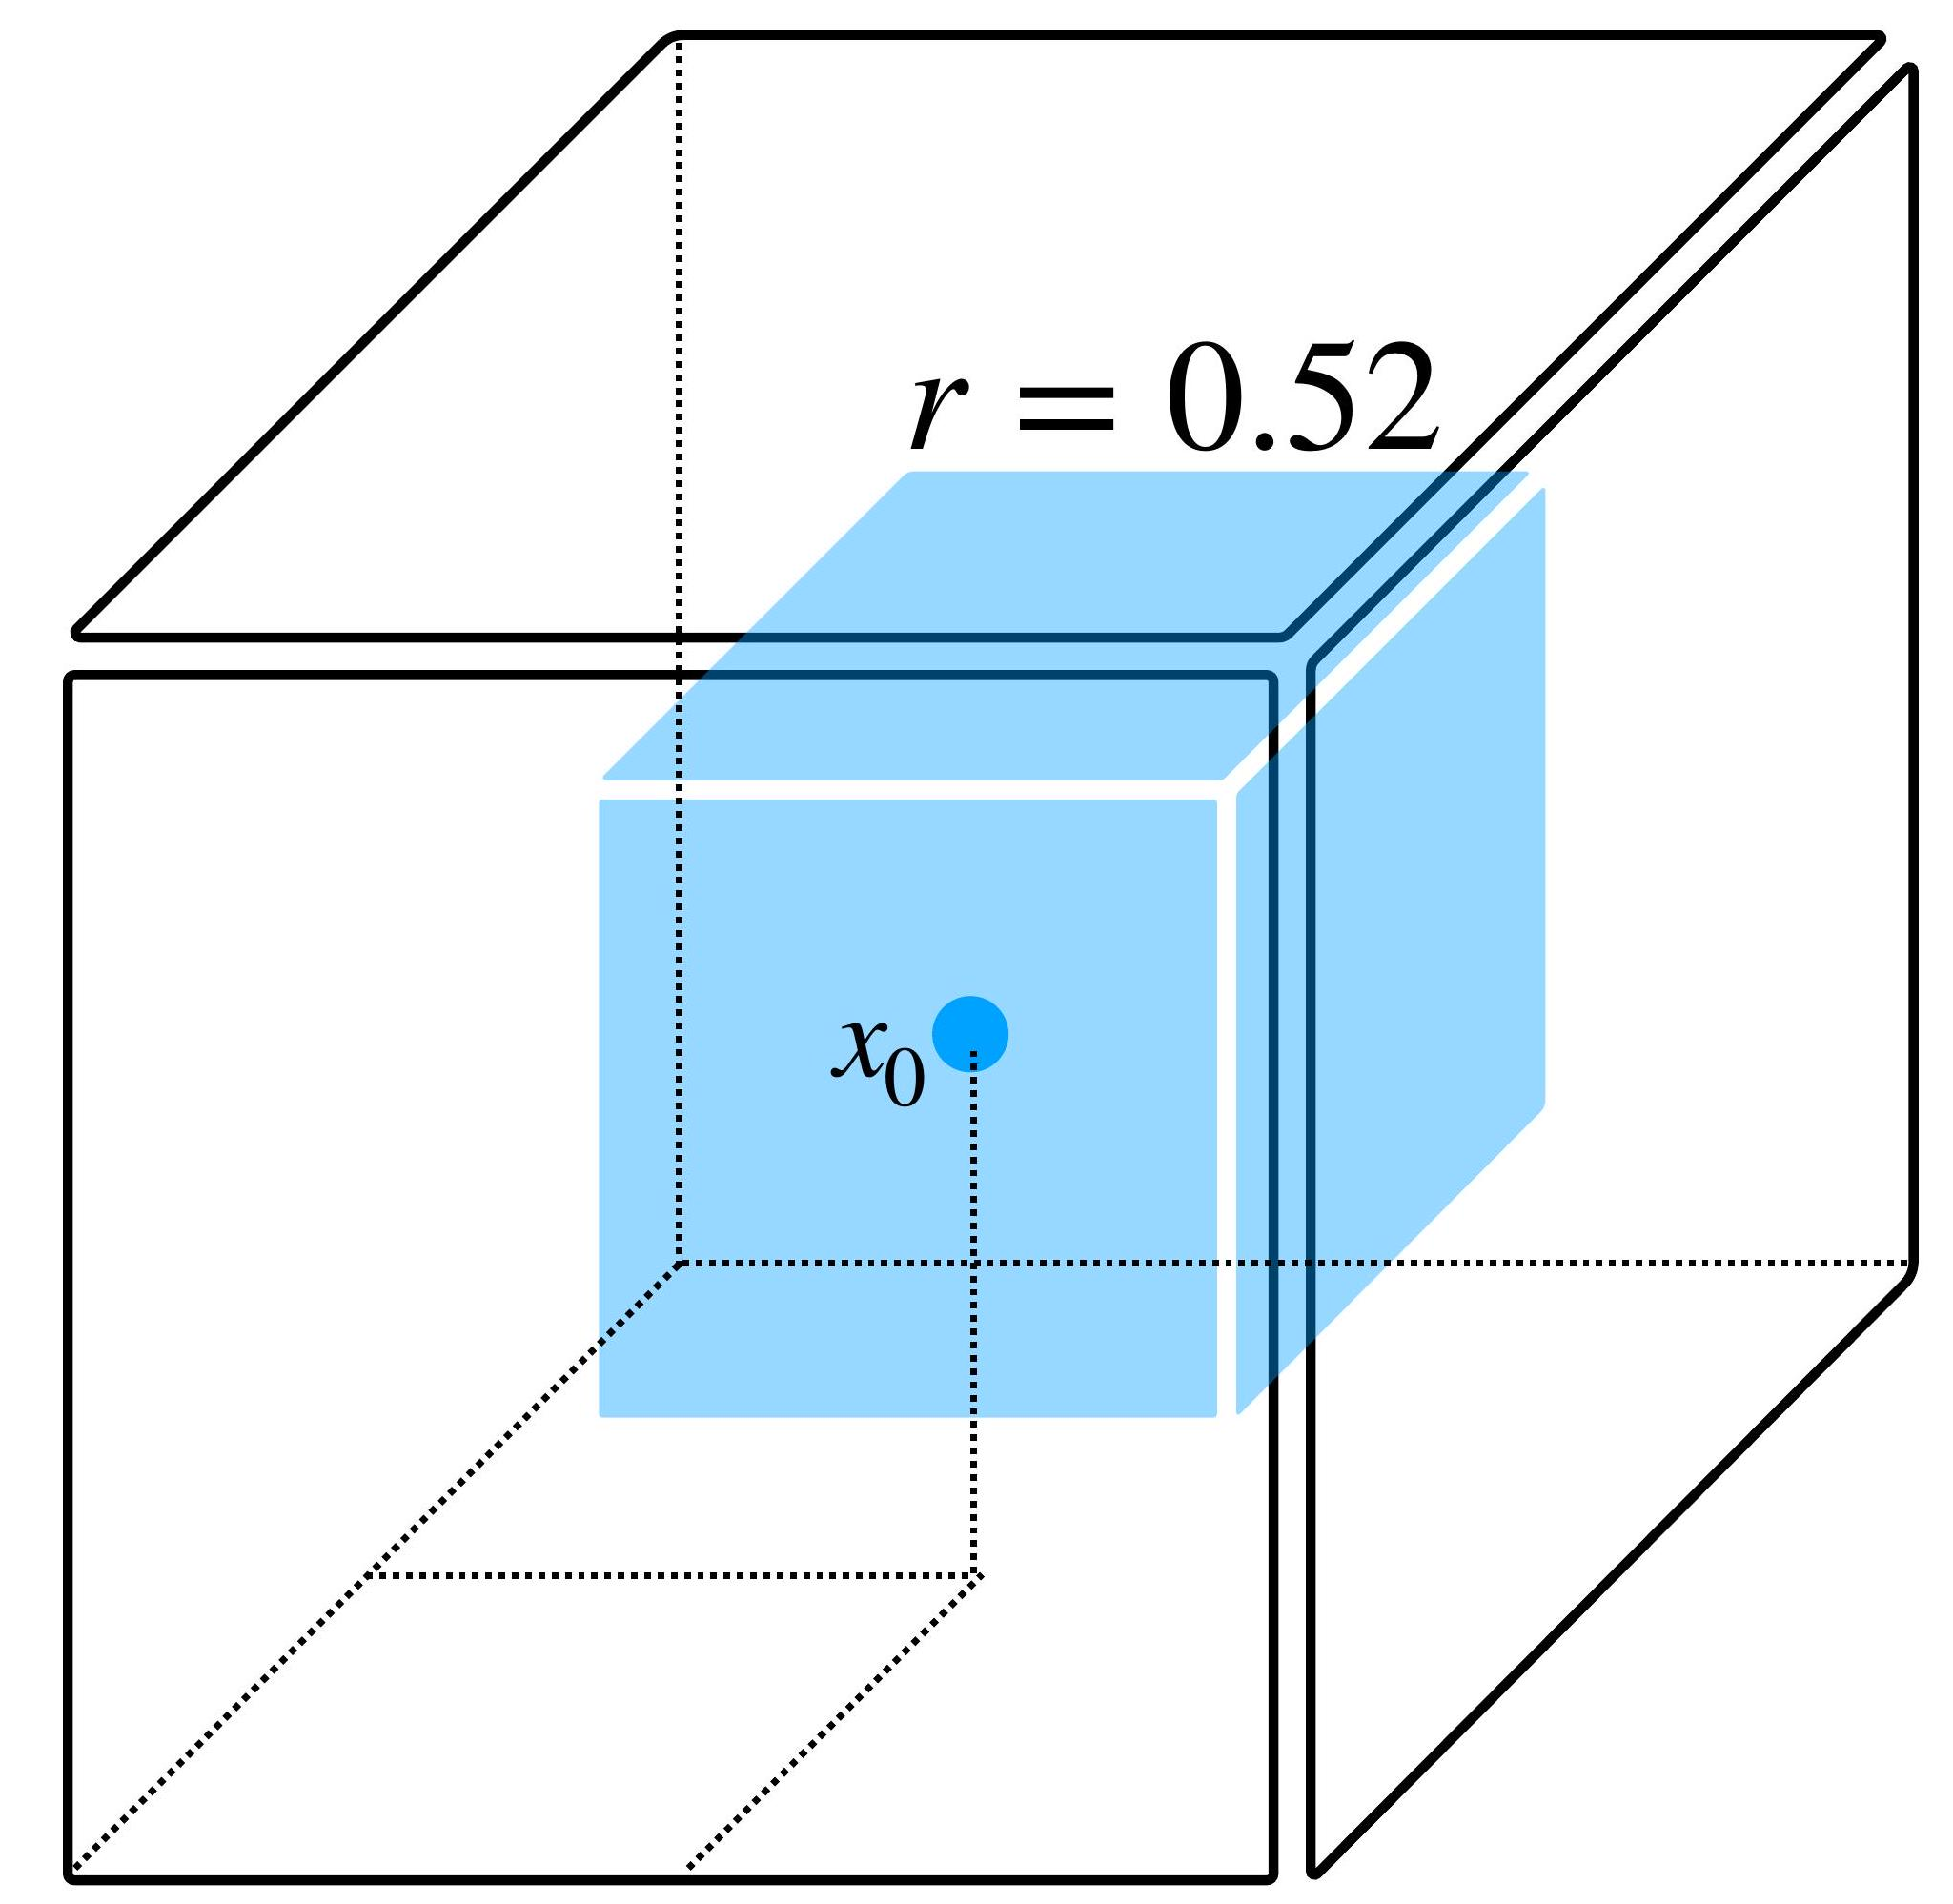
\includegraphics[width=0.2\columnwidth]{figures/dim_r=0_52.jpg}
    \text{\tiny{$\mathscr{X}=[0,1]^{d}$}}
\end{wrapfigure}

- Proof: $\mathbb{P}(x \notin \mbox{\mancube})=1-r^{d}$

$
\begin{aligned}
& \mathbb{P}\left(x_{i} \notin \mbox{\mancube}\ , \forall i \leq N\right)=\left(1-r^{d}\right)^{N} \\
& \mathbb{P}\left(\exists x_{i} \in \mbox{\mancube}\right)=1-\left(1-r^{d}\right)^{N}
\end{aligned}
$

- For $d=10, N=500$, $r \geq 0.52$


\subsection*{Generalization bound for 1-NN (I)}
- Setup: $(X, Y) \sim \mathscr{D}$ over $\mathscr{X} \times \mathscr{Y}=[0,1]^{d} \times\{0,1\}$

- Goal: Bound the classification error:

$
L(f)=\mathbb{P}_{(X, Y) \sim D}(Y \neq f(X))
$

- Baseline:

\begin{itemize}
  \item Bayes classifier: minimizes $L$ over all classifiers
\end{itemize}

$
f_{*}(x)=1_{\eta(x) \geq 1 / 2} \text { where } \eta(x)=\mathbb{P}(Y=1 \mid X=x)
$

\underline{Proof 1:}

\scalebox{0.7}{
$\begin{aligned}
    \eta(x)\geq1/2& \Longleftrightarrow\mathbb{P}(Y=1|X=x)\geq1/2  \\
    &\Longleftrightarrow\mathbb{P}(Y=1\mid X=x)\geq\mathbb{P}(Y=0\mid X=x) \\
    &\Longleftrightarrow1\in\arg\max_{y\in\{0,1\}}\mathbb{P}(Y=y|X=x) \\
    &\Rightarrow1_{\eta(x)\geq1/2}=\arg\max_{y\in\{0,1\}}\mathbb{P}(Y=y|X=x)=f_{*}(x)
\end{aligned}$
}

\begin{itemize}
  \item Bayes risk: represents the minimum probability of misclassification
\end{itemize}

$
L\left(f_{*}\right)=\mathbb{P}\left(f_{*}(X) \neq Y\right)\\=\mathbb{E}_{X \sim D_{X}}[\min \{\eta(X), 1-\eta(X)\}]
$

\underline{Proof 2:}

\scalebox{0.6}{
$
\begin{aligned}
& L(f_{*}) = \mathbb{E}_{(X, Y) \sim \mathscr{D}}[1_{f_{*}(X) \neq Y}] \\
& = \mathbb{E}_{X \sim \mathscr{D}_{X}}[\mathbb{E}_{Y \sim \mathscr{D}_{Y \mid X}}[1_{f_{*}(X) \neq Y} \mid X] 1_{\eta(X) \geq 1 / 2} + \mathbb{E}_{Y \sim \mathscr{D}_{Y \mid X}}[1_{f_{*}(X) \neq Y} \mid X] 1_{\eta(X) < 1 / 2}] \\
& = \mathbb{E}_{X \sim \mathscr{D}_{X}}[\mathbb{E}_{Y \sim \mathscr{D}_{Y \mid X}}[1_{1 \neq Y} \mid X] 1_{\eta(X) \geq 1 / 2} + \mathbb{E}_{Y \sim \mathscr{D}_{Y \mid X}}[1_{0 \neq Y} \mid X] 1_{\eta(X) < 1 / 2}] \\
& = \mathbb{E}_{X \sim D_{X}}[\mathbb{P}(Y=0 \mid X) 1_{\eta(X) \geq 1 / 2} + \mathbb{P}(Y=1 \mid X) 1_{\eta(X) < 1 / 2}] \\
& = \mathbb{E}_{X \sim \mathscr{D}_{X}}[\min \{\eta(X), 1-\eta(X)\}]
\end{aligned}
$
}

\subsection*{Generalization bound for 1-NN (II)}

- Assumption: $\exists c \geq 0, \forall x, x^{\prime} \in \mathscr{X}$ :

$
\left|\eta(x)-\eta\left(x^{\prime}\right)\right| \leq c\left\|x-x^{\prime}\right\|_{2}
$

$\Rightarrow$ Nearby points are likely to share the same label

- Claim:
$
\mathbb{E}_{S_{\text {train }}}\left[L\left(f_{S_{\text {train }}}\right)\right] 
\\\leq 2 L\left(f_*\right) +c \mathbb{E}_{S_{\text {train }}, X \sim \mathscr{D}_X}\left[\underbrace{\left\|X-\operatorname{nbh}_{S_{\text {train }}, 1}(X)\right\|}_{\text{geometric term}}\right] 
\\\leq 2 L\left(f_{*}\right)+4 c \sqrt{d} N^{-\frac{1}{d+1}}
$

% geometric term: average distance between a random point and its closest neighbor


- Interpretation:
\begin{itemize}
    \item For constant $d$ and $N \rightarrow \infty: \mathbb{E}_{S_{\text {train }}}\left[L\left(f_{S_{\text {train }}}\right)\right] \leq 2 L\left(f_{*}\right)$
    \item To achieve a constant error, we need $N \propto d^{(d+1) / 2}$ - curse of dimensionality
    \item Despite common belief: Interpolation method can generalize well
\end{itemize}


\subsubsection*{Proof (I)}
- We want to bound:

$
\mathbb{E}_{S_{\text {train }}}\left[L\left(f_{S_{\text {train }}}\right)\right]\\=\mathbb{E}_{S_{\text {train }}}\left[\mathbb{P}_{(X, Y) \sim \mathscr{D}}\left[f_{S_{\text {train }}}(X) \neq Y\right]\right]
$

- We first sample $N$ unlabeled examples $S_{\text {train }, X}=\left(X_{1}, \cdots X_{N}\right) \sim \mathscr{D}_{X}$, an unlabeled example $X \sim \mathscr{D}_{X}$ and define $X^{\prime}=\operatorname{nbh}_{S_{\text {train }, 1}}(X)$

- Finally we sample $Y \sim \eta(X)$ and $Y^{\prime} \sim \eta\left(X^{\prime}\right)$

$
\begin{aligned}
& \mathbb{E}_{S_{\text {train }}}\left[L\left(f_{S_{\text {train }}}\right)\right]\\
& =\mathbb{E}_{S_{\text {train }, X}, X \sim D_{X}, Y \sim \eta(X), Y^{\prime} \sim \eta\left(X^{\prime}\right)}\left[1_{Y \neq f_{S_{\text {train }}(X)}}\right] \\
& =\mathbb{E}_{S_{\text {train, } X}, X \sim \mathscr{D}_{X}, Y \sim \eta(X), Y^{\prime} \sim \eta\left(X^{\prime}\right)}\left[1_{Y \neq Y^{\prime}}\right] \\
& =\mathbb{E}_{S_{\text {train }, X}, X \sim \mathscr{D}_{X}}\left[\mathbb{P}_{Y \sim \eta(X), Y^{\prime} \sim \eta\left(X^{\prime}\right)}\left(Y \neq Y^{\prime}\right)\right]
\end{aligned}
$

\subsubsection*{Proof (II)}
- Consider two points $x, x^{\prime} \in[0,1]^{d}$.

- Sample their labels $Y \sim \eta(x)$ and $Y^{\prime} \sim \eta\left(x^{\prime}\right)$

- \underline{Claim}:

$
\mathbb{P}\left(Y^{\prime} \neq Y\right) \leq 2 \min \{\eta(x), 1-\eta(x)\}+c\left\|x-x^{\prime}\right\|
$

- Simple case: $x=x^{\prime}$

\scalebox{0.8}{
$
\begin{aligned}
\mathbb{P}\left(Y^{\prime} \neq Y\right) & =\mathbb{E}\left[1_{Y^{\prime} \neq Y} 1_{Y^{\prime}=1}+1_{Y^{\prime} \neq Y^{\prime}} 1_{Y^{\prime}=0}\right] \\
& =\mathbb{P}\left(Y^{\prime}=1\right) \mathbb{P}(Y=0)+\mathbb{P}\left(Y^{\prime}=1\right) \mathbb{P}(Y=0) \\
& =2 \eta(x)(1-\eta(x)) \\
& \leq 2 \min \{\eta(x), 1-\eta(x)\}
\end{aligned}
$
}

- Case 1:
$\mathbf{Y}=\mathbf{0} \quad (1-\eta(x)) \quad Y^{\prime}=1 \quad \eta(x)$

- Case 2:
$\mathrm{Y}=\mathbf{1} \quad \eta(x) \quad Y^{\prime}=0 \quad(1-\eta(x))$

\subsubsection*{Proof (III)}
\begin{itemize}
  \item General case:
\end{itemize}

\scalebox{0.8}{
$
\begin{aligned}
\mathbb{P}\left(Y \neq Y^{\prime}\right)= & \eta(x)\left(1-\eta\left(x^{\prime}\right)\right)+\eta\left(x^{\prime}\right)(1-\eta(x)) \\
= & \eta(x)(1-\eta(x))+\eta(x)\left(\eta(x)-\eta\left(x^{\prime}\right)\right) \\
& \quad+\eta(x)(1-\eta(x))+\left(\eta\left(x^{\prime}\right)-\eta(x)\right)(1-\eta(x)) \\
= & 2 \eta(x)(1-\eta(x))+(2 \eta(x)-1)\left(\eta(x)-\eta\left(x^{\prime}\right)\right) \\
& \leq 2 \eta(x)(1-\eta(x))+|(2 \eta(x)-1)|\left|\eta(x)-\eta\left(x^{\prime}\right)\right| \\
& \leq 2 \eta(x)(1-\eta(x))+\left|\eta(x)-\eta\left(x^{\prime}\right)\right| \\
& \leq 2 \eta(x)(1-\eta(x))+c\left\|x-x^{\prime}\right\| \\
& \leq 2 \min \{\eta(x), 1-\eta(x)\}+c\left\|x-x^{\prime}\right\|
\end{aligned}
$
}

\subsubsection*{Proof (IV)}
\scalebox{0.6}{
$
\begin{aligned}
\mathbb{E}_{S_{\text {train }}}\left[L \left(f_{\left.\left.S_{\text {train }}\right)\right]}\right.\right. & =\mathbb{E}_{S_{\text {train, }, X}, X \sim \mathscr{D}_{X}, Y \sim \eta(X), Y^{\prime} \sim \eta\left(X^{\prime}\right)}\left[1_{Y \neq f_{\text {train }(X)}}\right] \\
& =\mathbb{E}_{S_{\text {train, }, X}, X \sim \mathscr{D}_{X}, Y \sim \eta(X), Y^{\prime} \sim \eta\left(X^{\prime}\right)}\left[1_{Y \neq Y^{\prime}}\right] \\
& =\mathbb{E}_{S_{\text {train }, X}, X \sim D_{X}}\left[\mathbb{P}_{Y \sim \eta(X), Y^{\prime} \sim \eta(X)}\left(Y \neq Y^{\prime}\right)\right] \\
& \leq \mathbb{E}_{S_{\text {train }, X}, X \sim \mathscr{D}_{X}}\left[2 \min \{\eta(X), 1-\eta(X)\}+c\left\|X-X^{\prime}\right\|\right] \\
& \leq 2 L\left(f_{*}\right)+c \mathbb{E}_{S_{\text {train }}, X \sim \mathscr{D}_{X}}\left[\left\|X-\operatorname{nbh}_{S_{\text {train }}, 1}(X)\right\|\right]
\end{aligned}
$
}

\subsection*{Bound on the geometric term (I)}
- Consider a fresh sample $X \sim \mathscr{D}$ and denote by $p_{k}=\mathbb{P}\left(X \in\right.$ Box $\left._{k}\right)$

\begin{wrapfigure}{r}{0.4\columnwidth} 
    \centering
    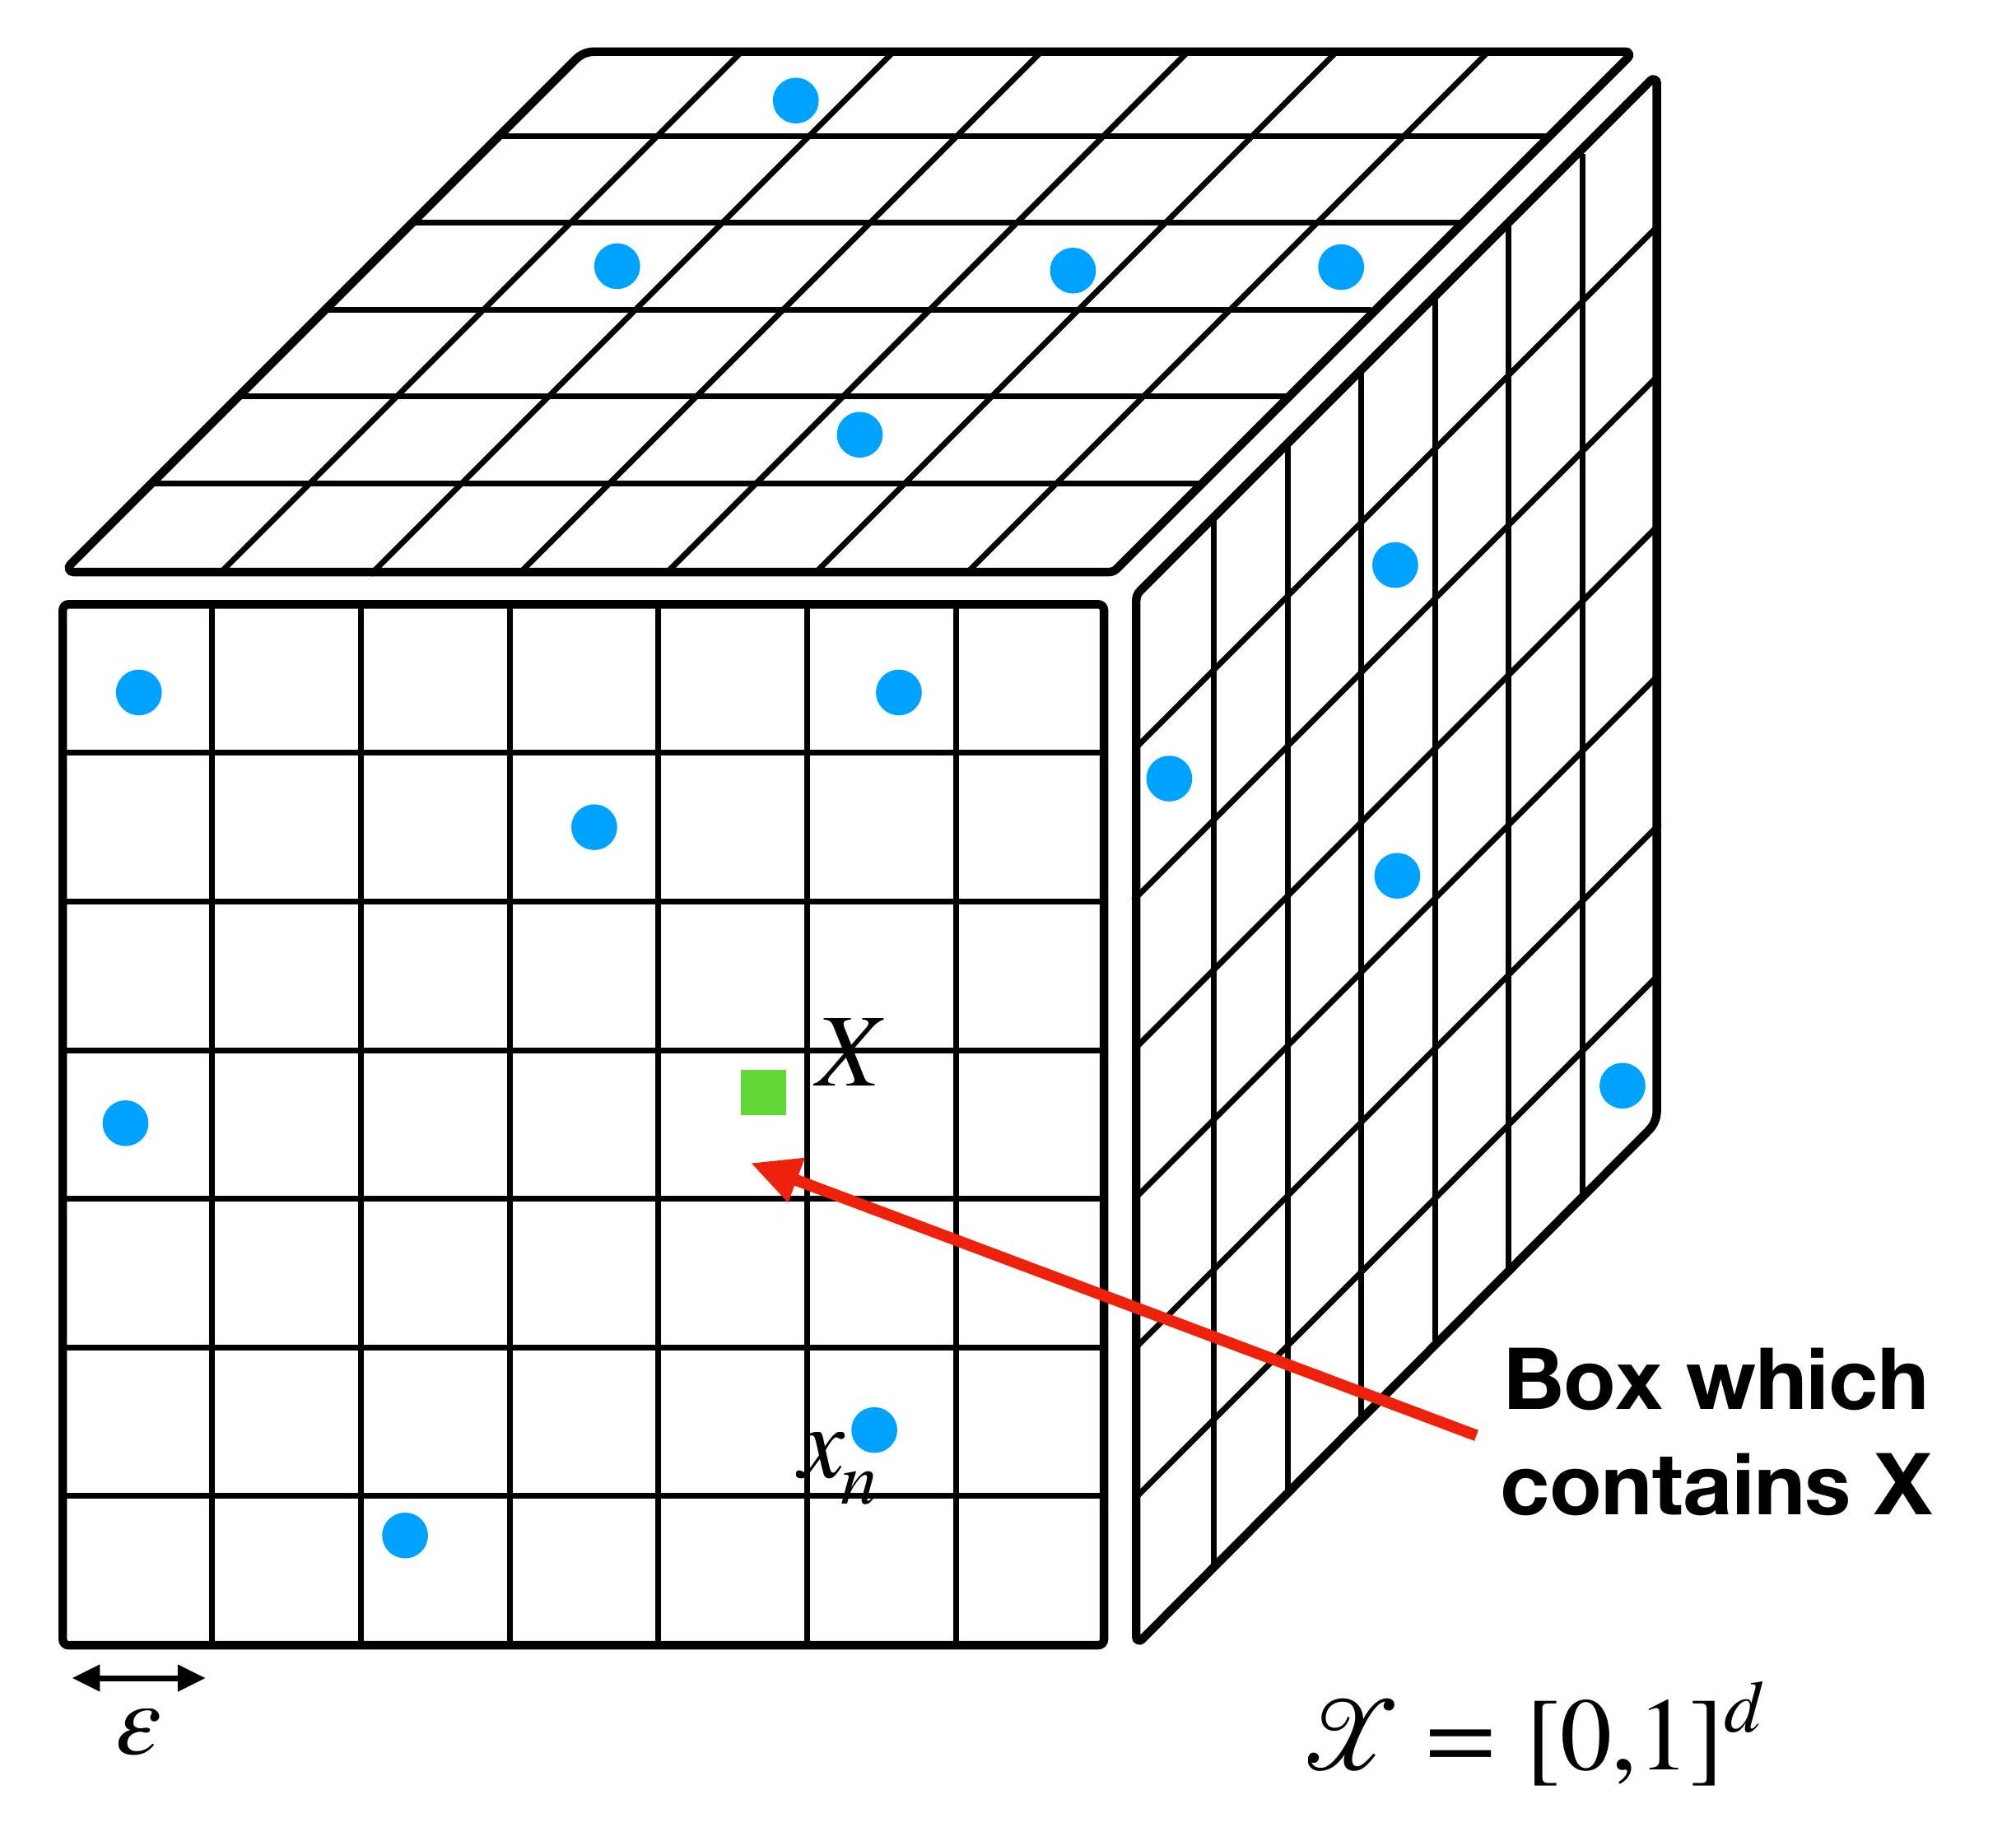
\includegraphics[width=0.4\columnwidth]{figures/dim_hypercube.jpg}
\end{wrapfigure}


- Consider the box which contains $X$. Two options:


\begin{itemize}
  \item The box contains an element of $S_{\text {train }}$ X has a neighbor in $S_{\text {train }}$ at distance at most $\sqrt{d} \varepsilon$
\end{itemize}

It happens with probability $1-\left(1-p_{k}\right)^{N}$

Proof: Consider the worst case: 

\begin{wrapfigure}{l}{0.2\columnwidth} 
    \centering
    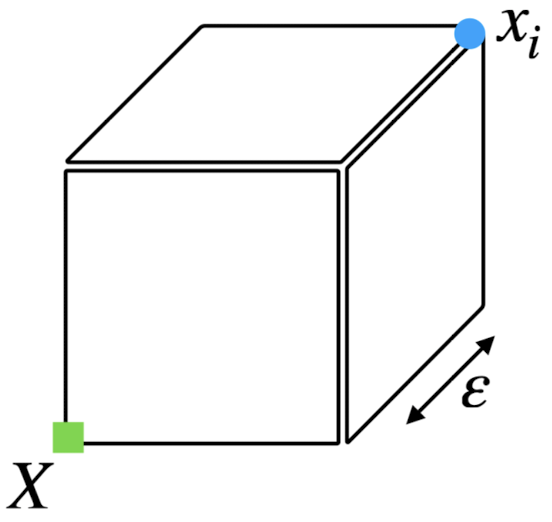
\includegraphics[width=0.2\columnwidth]{figures/dim_worst_case.png}
\end{wrapfigure}

$
\left\|X-x_{i}\right\|=\sqrt{\sum_{i=1}^{d} \varepsilon^{2}}=\sqrt{d} \varepsilon
$

\begin{itemize}
  \item There is no element of $S_{\text {train }}$. The nearest neighbor of $\mathrm{X}$ can be at worst at a distance $\sqrt{d}$ It happens with probability $\left(1-p_{k}\right)^{N}$
\end{itemize}



\subsection*{Bound on the geometric term (II)}
$\mathbb{E}[\|X-\mathrm{nbh}(X)\|] \\\leq \sum_{k} p_{k}\left[\left(1-p_{k}\right)^{N} \sqrt{d}+\left(1-\left(1-p_{k}\right)^{N}\right) \sqrt{d} \varepsilon\right]$

- Claim: The bound is derived by optimizing over $p_{k}$ and $\varepsilon$

- Intuition:

\begin{itemize}
  \item If $p_{k}$ is large: it is likely that we pick that box but it is also likely that we find a training point in that box
  \item If $p_{k}$ is small, we are generally safe, as by its definition, this scenario occurs infrequently
\end{itemize}


\subsection*{Nearest Neighbors is a local averaging method}
- Local averaging methods aim to approximate the Bayes predictor directly - without the need for optimization

- This is achieved by approximating the conditional distribution $p(y \mid x)$ by some $\hat{p}(y \mid x)$ These "plug-in" estimators are:

\begin{itemize}
    \item $f(x) \in \arg \max \hat{\mathbb{P}}(Y=y \mid x)$ for classification with the $0-1$ loss $y \in \mathcal{Y}$
  \item $f(x)=\hat{\mathbb{E}}[Y \mid x]=\int_{\mathscr{y}} y \hat{p}(y \mid x) d y$ for regression with the square loss
  
\end{itemize}

- In the case of nearest neighbors:

$
\hat{p}(y \mid x)=\sum_{n=1}^{N} \hat{w}_{n}(x) 1_{y=y_{n}}
$

where $\hat{w}(x)=1 / k$ for the $k$ nearest neighbors ( 0 otherwise)

\subsection*{Recap}
\begin{itemize}
  \item Curse of dimensionality: as $d \nearrow \infty$, it is harder to define local neighborhoods

  \item For $N \rightarrow \infty, 1-\mathrm{NN}$ is competitive with Bayes classifier

  \item $N$ needs to scale exponentially in $d$ to achieve the same error

\end{itemize}